Field-Programmable Gate Arrays (FPGAs) are readily available, multi-sourced components which have a proven place in development, small-scale production, and even large-scale production runs. 
Its impressive properties, such as high computational speed and intrinsic parallelism, are crucial in most of the experiments and applications performed nowadays.
Many application programs demand more processing power than can be supplied by conventional processing resources. Many of these programs have a kernel which is responsible for a significant fraction of the total execution time of the program. 

\subsection{Architecture}
FPGAs consist of an array of programmable logic blocks of potentially different types, including general logic, memory and multiplier blocks, surrounded by a programmable routing fabric that allows blocks to be programmably interconnected. The array is surrounded by programmable input/output blocks that connect the chip to external devices\cite{fpgaStructureBook}.

\begin{figure}[H]
    \centering
    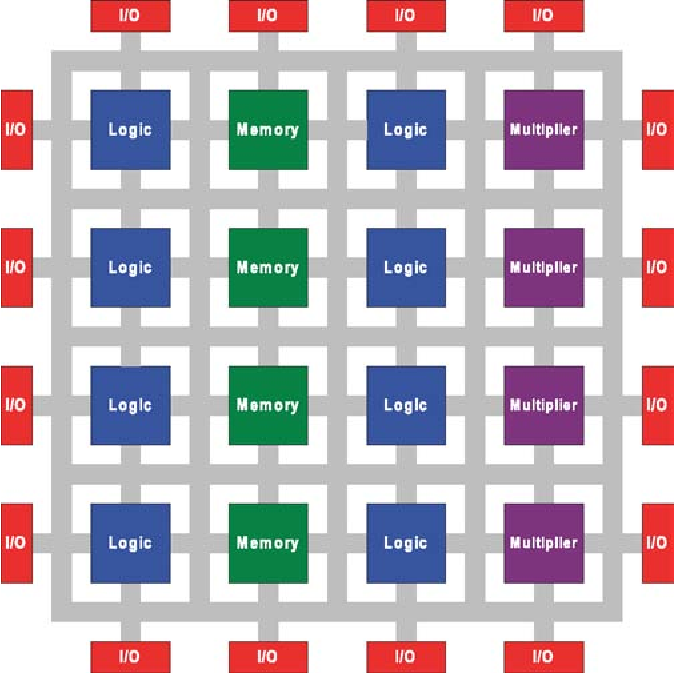
\includegraphics[width=0.5\linewidth]{img/fpgaStructure.png}
    \caption{Basic FPGA structure\cite{fpgaStructureBook}}
    \label{fig:fpgaStructure}
\end{figure}

\subsection{FPGA as hardware accelerators}
FPGAs usually operate at lower clock frequencies than ASICs (Application Specific Integrated Circuits) and ASSPs (Application-Specific Standard Products), but they are very customizable and present multiple advantages:
\begin{itemize}
    \item Implementing wider parallelism in hardware
    \item Easily changing the size of data
    \item Provides an easy and inexpensive way to modify the neural network.
    \item Experimentation with alternative circuits makes them very attractive for both prototyping and new products.
\end{itemize}
The main disadvantage when it comes to using FPGAs is the price. FPGAs are more expensive than the majority of widely used microprocessors. For some applications, microprocessors also perform better. Thus, FPGAs are relevant for only a set of high-performance computations and algorithms.

Hardware accelerators are, as a rule, non-autonomous circuit that has to interact with some other circuits, and yields better performances as more items are handled in parallel.